	\FloatBarrier
	\begin{figure}[b!]
		\centering
		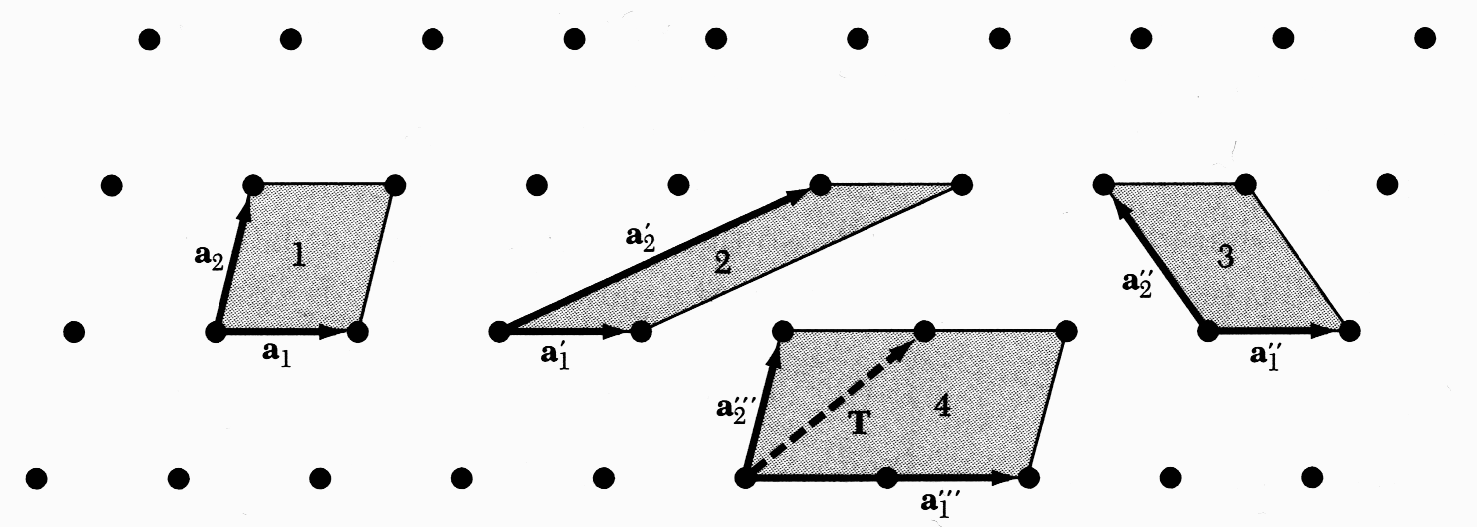
\includegraphics[width=.9\linewidth]{andere_bilder/basis_2dim.png}
		\caption{Some two dimensional unit cells with different basis vectors. The cells 1,2 and 3 are primitive unit cells, but 4 
%		isn't because it is twice as big as 1.
		is not because its volume is twice as big as, for example, the parallelogram number 1. For a primitive cell it must be verified that the volume is as small as possible in order to reproduce the lattice when repeated in space in all directions considered. 
		(Picture from\cite{Kittel})}\label{basis_2dim}
	\end{figure}
	%crystals, bulk, surfaces, band structures. What they are? Talk about the Brillouin zones and the real and reciprocal space. How are they related to each other?
%	-unendliches Gitter-> bulk
%	-Wigner-Seitz->primitive einheitszelle
%	-Bravaisgitter
%	-sc,bcc,fcc,diamand struktur
%	-millersche indizes
%	-zinkblendestruktur
%	-reziproker raum
%	-Brillouin zonen
%	-band structure
%	-surfaces

%	In solid state physics, the characteristics of the inner part of a finite crystals are approximated by infinite lattices. This part of a solid, where the surfaces are not regarded, is called the bulk. 
	A crystal structure describes the arrangement of atoms in a crystalline material. The atoms out of which a crystal is made, maintain a symmetric pattern repeating itself into the three spatial dimensions. 
	
%	\subsubsection{General description of the crystal structure}
	For this reason, to describe the crystal structure, one needs a basis, which can start at any atom $i$ in the lattice, in order to form a unit cell. For a three dimensional crystal, we need a three dimensional lattice and to describe the crystal lattice we introduce three primitive translation vectors $\fata_1,\fata_2$ and $\fata_3$. These vectors indicate the directions where to the atom $i$ of the crystal, which holds the coordinates $x_i, y_i $ and $z_i$, must be replicated in order to compose the whole crystalline structure. The crystal translation vector $\boldsymbol{R}_i$ is then defined as 
%	three basis vectors in need $\fata_1,\fata_2, \fata_3$ so that the structure is given by:
	\begin{equation} \label{vector}
		\boldsymbol{R}_i = x_i \fata_1 + y_i \fata_2 + z_i \fata_3
	\end{equation}
	There are different ways to choose the basis set for the unit cells, some possible choices for a two dimensional lattice are illustrated in figure \ref{basis_2dim}. In this figure one can also see some unit cells, shown in grey areas, that, with the exception of 4, are primitive unit cells.
%	Some examples of how to choose a possible basis set for a two dimensional lattice are illustrated in figure \ref{basis_2dim}.
%	-Bravaisgitter
%	-sc,bcc,fcc,diamand struktur
	
%	-Wigner-Seitz->primitive einheitszelle
	A primitive cell is a unit cell which includes the smallest possible number of atoms and possesses the minimum volume whose lattice vectors describe the crystal lattice.  
%	with minimal volume.
	Its basis vectors do not include atoms like they are in cell 4 in figure \ref{basis_2dim},
%	this one even has the double volume of cell 1. 
	which has, as we can see, twice the volume of cell example number 1.
	There are many ways of choosing the basis, the parallelograms 1, 2 and 3 are examples of primitive cells. 
	The smallest primitive cell is the Wigner-Seitz cell and is defined as the unit cell, which contains one single atom that is placed at its center. In 2D it can be constructed by linking the basis atom with all next neighbors by a line, put a straight line at the middle of each line, and then the space around the basis atom is the Wigner-Seitz cell. 
\subsection{Crystal surfaces.}	
	\subsubsection{The zinc-blende crystal and its (001) cleavage} \label{cleavage_fcc}
%	Due to the point symmetry, there are just 14 different periodical lattice types in three dimensional space. They are called Bravais lattices. One of them is the most general lattice, because it has three different long basis vectors with three different angles. This leaves 13 special cases.
%	For this thesis, it's the fcc cubic lattice shown in figure \ref{fcc} I will contemplate, because it's nearly the same as the diamond lattice. The basis vectors are written in the tabular next to the drawing of the unit cell and so are the coorinates of the basis atoms.
	\begin{figure}[b!]
		\begin{minipage}[c]{.38\linewidth}
			\centering
			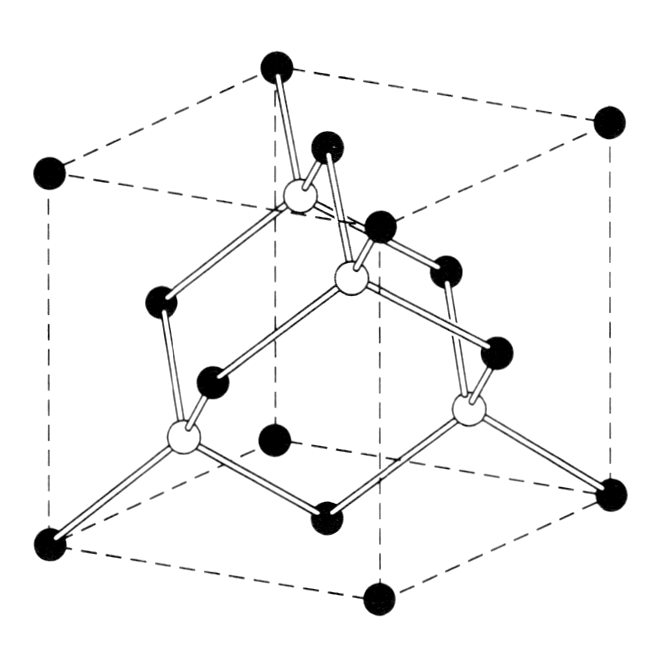
\includegraphics[width=.9\linewidth]{andere_bilder/diamond.png}
		\end{minipage}
		\hfill
		\begin{minipage}[c]{.25\linewidth}
			\centering
			\begin{tabular}{c c c c} 
				\hline
				& \textbf{x} & \textbf{y} & \textbf{z}\\ 
				\hline 
				\vspace{0.2cm} 
				$\fata_1$ & 0 & $\frac{a}{2}$ & $\frac{a}{2}$ \\
				\vspace{0.2cm}
				$\fata_2$ & $\frac{a}{2}$ & 0 & $\frac{a}{2}$ \\
				\vspace{0.2cm}
				$\fata_3$ & $\frac{a}{2}$ & $\frac{a}{2}$ & 0 
			\end{tabular}	
		\end{minipage}
		\hfill
		\begin{minipage}[c]{.33\linewidth}
			%			\textbf{fcc}
			%			\begin{tabular}{c c c c} 
			%				\hline
			%				& \textbf{x} & \textbf{y} & \textbf{z}\\ 
			%				\hline 
			%				\vspace{0.2cm} 
			%				basis atom & 0 & 0 & 0 \\
			%			\end{tabular}	
			%			\vfill
			%			\textbf{diamond} 
			\begin{tabular}{c c c c} 
				\hline
				& \textbf{x} & \textbf{y} & \textbf{z}\\ 
				\hline 
				\vspace{0.2cm}
				basis atom & 0 & 0 & 0 \\
				\vspace{0.2cm}
				basis atom & $\frac{a}{4}$ & $\frac{a}{4}$ & $\frac{a}{4}$
			\end{tabular}	
		\end{minipage}
		\caption{This is the cubic diamond lattice on the left (Picture from\cite{Kittel}). In the middle there are the basis lattice vectors of the primitive unit cell for a diamond crystal, and on the right there are the basis atoms for fcc and diamond.
			%		As one can see, the diamond structure just has an additional atom at $\frac{a}{4},\frac{a}{4},\frac{a}{4}$ as basis.
		}\label{fcc}
	\end{figure}
	Now we introduce the concept of Bravais lattices. A Bravais lattice is defined by an infinite number of discrete points which are arranged in a translational symmetric way. It is described by a vector $\boldsymbol{R}$ given by \eqref{vector}, whereat the points are generated by integer translations. 
	Each point can be connected to a basis of one or more atoms.
	
	In three dimensional space, there are 14 different types of Bravais lattices. In this thesis we work with the so called face-centered cubic (fcc) lattice with a basis composed of two different species of atoms.
	This lattice is also known as zinc-blende structure which is similar to the diamond structure whose basis contains two identical basis atoms at $(0,0,0)$ and $(\frac{a}{4},\frac{a}{4},\frac{a}{4})$.
%	It is the structure of several important  \marginpar{cite} semiconductors. 
	Note that this structure can be understood as two fcc lattices which are shifted in respect to each other.
	The coordinates of the atoms and the primitive basis vectors can be seen in figure \ref{fcc} and as well as a picture of the zinc-blende structure.
	
%	 On the other hand, the zinc-blende structure, which HgTe is growing in, is nearly the same as the diamond structure, with the only difference namely that the basis atoms are of a different kind. In figure \ref{hgte_diamond001} is a picture of this lattice. The grey atoms are at the same place as the black ones in figure \ref{fcc}.	
%	-millersche indizes

%	It is important to know, onto which plane in a crystal one is looking while doing experiments. 
 	
	Crystals are grown plane by plane in different directions. 
	Those planes can be identified by the so-called miller indices ($hkl$).
%	These numbers are obtained by taking the reciprocal of the integers, with which one has to multiply the basis vectors, so that they are intercepting with the plane, and find the smallest integers for which the fractions have the same ratio.
	The integers $h$, $k$ and $l$ are obtained by multiplying each basis vector with a number, so that it touches the plane, inverting these numbers $x$, $y$ and $z$ in respect to multiplication, in other words, writing them in a fractions denominator, whereby these fractions are in the same ratio as the miller indices, and finally expand the fractions until they are integers indivisible by another integer. The connection between the miller indices and the numbers $x$, $y$ and $z$ is
	\begin{equation}
		h : k : l = \frac{1}{x} : \frac{1}{y} : \frac{1}{z}
	\end{equation}
	Some examples can be seen in figure \ref{millersche_indizes}.
	\begin{figure}[tbp]
		\centering
		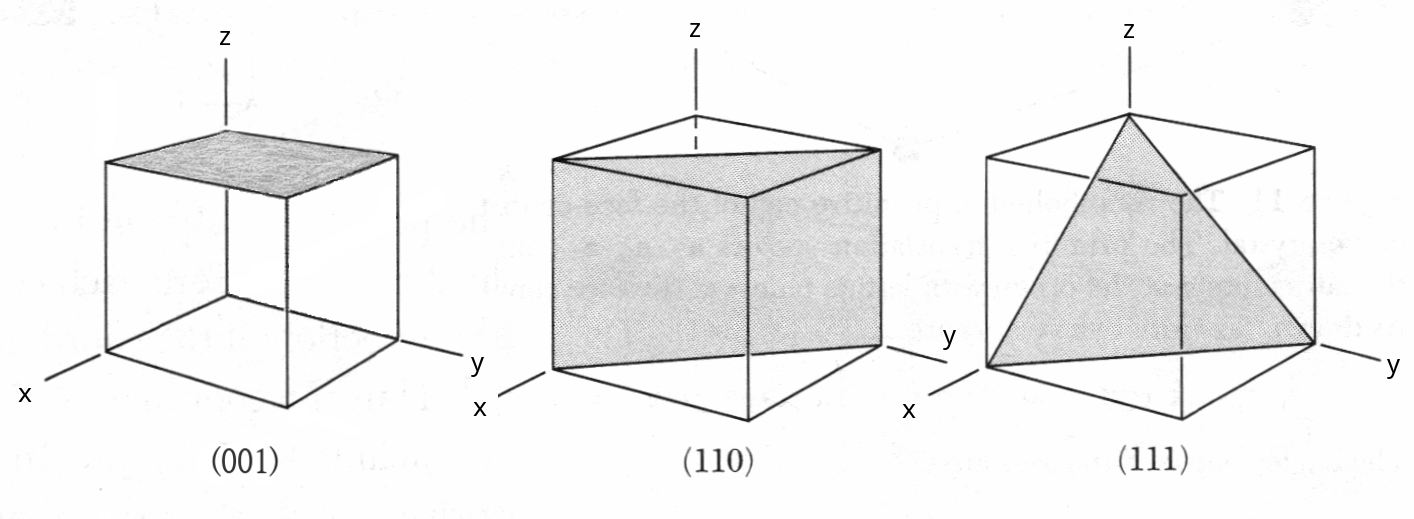
\includegraphics[width=.8\linewidth]{andere_bilder/millersche_indizes_less.png}
		\caption{Important planes in cubic crystals with their indices. At the left, there is the (001) which is analyzed for HgTe zinc-blende structure in this thesis. (Picture from\cite{Kittel})} \label{millersche_indizes}
	\end{figure}
%	-zinkblendestruktur
	
	In this thesis we will focus on the study of mercury telluride which is a crystal with two basis atoms Hg and Te, arranged in a zinc-blende structure. 
	In order to perform the calculations, we are focusing on HgTe at the diamond (001) cleavage, which is the top plane illustrated in figure \ref{millersche_indizes}. It is convention not to use the unit cell in the left of figure \ref{hgte_diamond001}, but to rotate the basis by $45^{\circ}$, like in the middle and the right of the same figure. This has the advantage, that the unit cell contains less atoms. 
	%which means less computational effort. \marginpar{cite misses}
	\begin{figure}[h!]
		\begin{minipage}[c]{.32\linewidth}
			\centering
			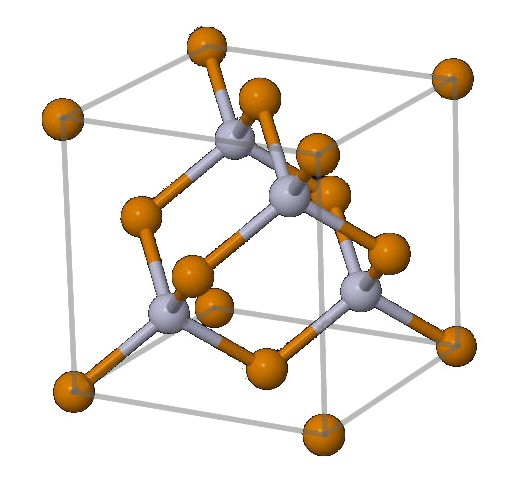
\includegraphics[width=0.9\linewidth]{andere_bilder/zinc_blende.jpg}
		\end{minipage}
		\hfill
		\begin{minipage}[c]{.32\linewidth}
			\centering
			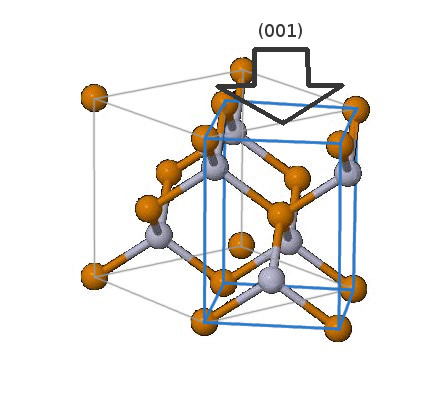
\includegraphics[width=\linewidth]{andere_bilder/zinc_blende_45degree.jpg}
		\end{minipage}
		\hfill
		\begin{minipage}[c]{.32\linewidth}
			\centering
			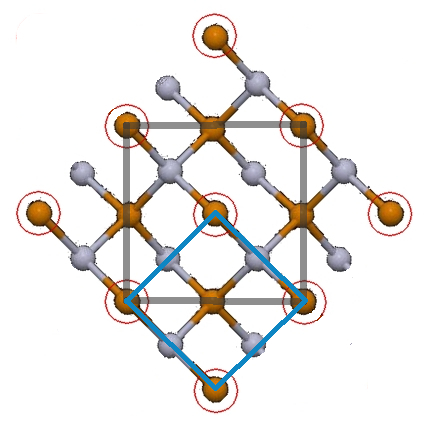
\includegraphics[width=.9\linewidth]{andere_bilder/001_plane_2.jpg}
		\end{minipage}
		\caption{Left: zinc-blende structure, two different kinds of atoms are labeled as Te (orange) and Hg (grey), note that this is not a primitive unit cell. Middle: rotation of basis by $45^\circ$, so that the new unit cell is the blue cuboid. Right: the top view. The red circles mark the atoms at the top, the blue lines are the small cell with length $\frac{a}{\sqrt{2}}$. The grey large square represents the (001) plane of the old unit cell.} \label{hgte_diamond001}
	\end{figure}
	The lattice vectors for diamond(001) are given by
	\begin{align} \label{001_basis}
		\fata_1&=\frac{a}{\sqrt{2}} \hat{\textbf{x}}; &
		\fata_2&=\frac{a}{\sqrt{2}} \hat{\textbf{y}}; &
		\fata_3&=a \hat{\textbf{z}}
	\end{align}
	where $a$ is the lattice constant of the crystal \cite{Graz} illustrated in the to the right in figure \ref{hgte_diamond001}. 
%	Later I will not use just $a$ for the z-direction, but $L$ which is composed of the slab thickness and the vacuum thickness on top of the surface. 
	In our case the basis atoms are at
	\\
	\begin{center}
		\begin{tabular}{c c c c} 
			\hline
			& \textbf{x} & \textbf{y} & \textbf{z}\\ 
			\hline 
			\vspace{0.2cm} 
			atomic species 1 & 0 & 0 & 0 \\
			\vspace{0.2cm}
			atomic species 2 & $\frac{a}{2\sqrt{2}}$ & 0 & $\frac{a}{4}$ \\
			\vspace{0.2cm}
			atomic species 1 & $\frac{a}{2\sqrt{2}}$ & $\frac{a}{2\sqrt{2}}$ & $\frac{a}{2}$ \\
			\vspace{0.2cm}
			atomic species 2 & 0 & $\frac{a}{2\sqrt{2}}$ & $\frac{3a}{4}$
		\end{tabular}
	\end{center}	
%	-reziproker raum
%	-Brillouin zonen
%	-band structure
	\FloatBarrier
	\subsubsection{Reciprocal lattice and first Brillouin zone.} \label{Brillouin_zone}
%		The reciprocal lattice of a Bravais lattice is the set of all wave vectors $\K$, which is produced by plane waves together with the periodicity of a given Bravais lattice.  
%		The relation between the vectors $\R$, which describe the given Bravais lattice, and the wave vectors $\K$ is
		The reciprocal lattice is defined as the Fourier transform of the direct Bravais lattice in real space. This transformation is mathematically equivalent to
		\begin{equation} \label{exp}
		e^{i \K \cdot \R} = 1.
		\end{equation}
		where $\K$ is the set of wave vectors in reciprocal space and $\R$ is defined as in eq. \ref{vector}.
		Consequently, every direct lattice has a corresponding reciprocal lattice which in addition, is a Bravais lattice too, since the Fourier transform acts within a group of discrete symmetries.		
%		A reciprocal lattice is only defined in respect to its Bravais lattice. The consequence is, that the reciprocal lattice is a Bravais lattice itself. Its vectors can generally be defined as:
		The primitive translation vectors of the reciprocal lattice can be obtained from eq. \eqref{exp} and their basis vectors are in three dimensional space related to the direct lattice vectors as
		\begin{align}
			\bb_1 &= \frac{2\pi}{V}(\fata_2 \times \fata_3); &
			\bb_2 &= \frac{2\pi}{V}(\fata_3 \times \fata_1); &
			\bb_3 &= \frac{2\pi}{V}(\fata_1 \times \fata_2)
		\end{align} 
		with $V=\fata_1 \cdot \fata_2 \times \fata_3$ being the volume of the primitive unit cell in real space.
		 
		The primitive Wigner-Seitz cell in the reciprocal space is called the first Brillouin zone. 
%		It is constructed similar and it has so called super symmetric points.
		The principle of constructing the first Brillouin zone is the same as for the earlier described Wigner-Seitz cells construction. The points, who stand out as high-symmetry points of the Brillouin zone, are marked by letters like K, L, U etc. The center of the Brillouin zone which happens to also be the origin of the Fourier space, is marked with the greek letter $\Gamma$.  
		The first Brillouin zone of the fcc and diamond crystal is shown in figure  \ref{brillouin_zone}.		
%		Since the zinc-blende structure is important for this thesis, it is good to know, that the reciprocal vectors of an fcc lattice are the primitive vectors of a bcc lattice but with a different length:

%		\begin{align} \label{fcc_reciprocal_vectors}
%			\bb_1 &= \frac{2\sqrt{2}\pi}{a} \hat{\textbf{x}} ;&
%			\bb_2 &= \frac{2\sqrt{2}\pi}{a} \hat{\textbf{y}} ;&
%			\bb_3 &= \frac{2\pi}{a} \hat{\textbf{z}}	
%		\end{align}

%	\begin{figure}[tbp]
%		\centering
%		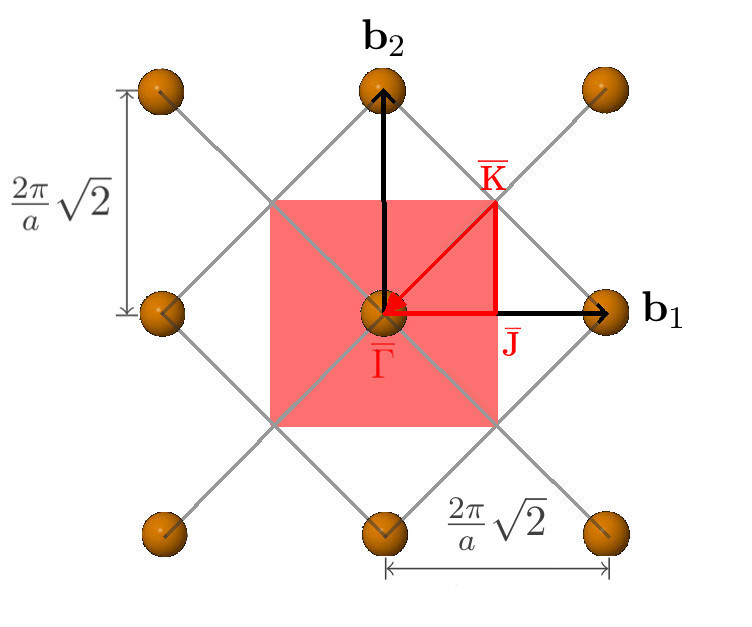
\includegraphics[width=.5\linewidth]{001_reciprocal_plane.jpg}
%		\caption{The light red region is the first Brillouin zone. The red line is the \textbf{k}-path for obtaining the band structure by calculating the dispersion relation. (Picture like in \cite{Graz})}\label{brillouin_zone_001}
%	\end{figure}
%		For calculating band structure of the bulk, one has to go a certain path along the symmetric points. 
%		But, in order to calculate the surface states of the HgTe, one has to choose which cleavage should be regarded. This also means $\Gamma$, X, L etc. of the 3D Brillouin zone cannot be used. Instead the super symmetric points of the 2D Brillouin zone must be taken. For the (001) plane those \textbf{k}-points, which are also illustrated in figure \ref{brillouin_zone_001},  are:
		
		The bulk band structure (see figure \ref{bulk_band_structure}), which gives the total energy in respect to the momentum, can now be seen as a one dimensional representation of a certain path which follows the high-symmetry points in the first Brillouin zone. 
		
		For the 2D periodic crystal slab, which grows in (001) direction, a two dimensional path can be taken along the high-symmetry points $\overline{\Gamma}$, $\overline{\text{J}}$ and $\overline{\text{K}}$. These points can be represented in terms of the reciprocal vectors $\bb_1$ and $\bb_2$:
		\begin{align} \label{2D-BZ-points}
			\overline{\Gamma}&= 0;&
			\overline{\text{J}} &= \frac{1}{2} \bb_1 ;&
			\overline{\text{K}}&= \frac{1}{2} \bb_1 + \frac{1}{2} \bb_2 
		\end{align}
		Therefore the 2D Brillouin zone, which corresponds to the slab, is like the projection of the 3D Brillouin zone into a plane which is defined by the vector $\bb_3$. 
	\begin{figure}[t!]
		\centering
		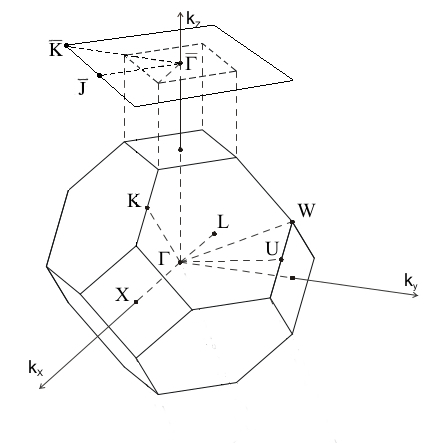
\includegraphics[width=.5\linewidth]{andere_bilder/brillouin_zone_001_2.jpg}
		\caption{First Brillouin zone of a fcc and diamond lattice. 
			%		In addition, there is the (001) plane at the top, which is a 2D Brillouin zone. The super symmetric points are marked with Latin letters and the one in the center with a $\Gamma$. 
			The plane at the top shows the 3D Brillouin zone projected in (001) direction, which is also defined by the vector $\boldsymbol{b}_3$. This corresponds to the first Brillouin zone in the 2D lattice. The high symmetry point are marked with latin letters, whereby the ones in the two dimensional Brillouin zone additionally have a bar and the point of origin is marked with a $\Gamma$, a bar is added for the one in the 2D Brillouin zone.  
			%		The points at the plane are additionally marked with a bar to distinguish them from the 3D Brillouin zone's points. 
			(Picture originally from\cite{aluminium})}\label{brillouin_zone}
	\end{figure}	
%		in respect to the reciprocal basis vectors \eqref{fcc_reciprocal_vectors}. 
%		For calculating the dispersion relation $E(k)$ of this plane, one has to go the along the red line in figure \ref{brillouin_zone_001}.
	%	-surfaces
	\subsubsection{Surface modeling} \label{surface_modeling}
%		In order to perform calculations for the surface states and properties, there are certain points about how to model the surface conditions correctly for getting physically correct results. Beginning with the boundary conditions, the bulk has 
%%		The way of calculating the dispersion relation was already explained in \ref{Brillouin_zone}, but after knowing the crystal and surface structure of HgTe in \ref{cleavage_fcc} I still didn't discuss how to exactly simulate the surface and the bulk.  
%%		
%%		The boundary conditions for the bulk are
%		infinite repetition in all three space directions. 
%		
%		In contrast, the surface has infinite repetition in two directions, here where the (001) plane is normal to the z-direction, thats the boundary condition in x- and y-direction for the surface calculations. But in the z-direction, thus the third direction, there is no repetition.
		The main goal of this thesis is to simulate the evolution of the topological surface states of HgTe. Therefore we first need to introduce the concept of surfaces and then simulate the (001) surface for an ideal slab. 
		
		The bulk is a model of a crystal which does not consider surfaces. For us, the most important difference are the boundary conditions. The bulk has periodic boundary conditions in all three spacial directions, but the slab has these in just two directions, in particular the x and y direction. Thus $k_z$ is no longer a good quantum number.  How this direction is simulated is explained in the following paragraphs. 
%		the termination of the crystal must be simulated. 
	\paragraph{Terminations}
	\begin{wrapfigure}{r}{0.3\linewidth}
		\centering
		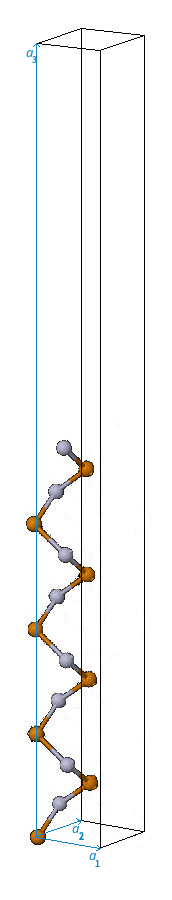
\includegraphics[width=0.6\linewidth]{andere_bilder/hgte_16layer_supercell_2.jpg}
		\caption{Supercell with 16 layers and additional space at the top, representing the vacuum. Basis vectors $\fata_1$, $\fata_2$ like in eq. \ref{001_basis}, $\fata_3$ with additional vacuum thickness.} \label{16layer_supercell}
		\vspace{-1cm}
	\end{wrapfigure} 	
%		One has to regard two surfaces at the bottom and at the top of the crystal in z-direction, which means it can be terminated by the same atoms, Te or Hg at the bottom and at the top, or it can be terminated by two different atoms, for example Te at the bottom, Hg at the top.
%		The first possibility is symmetric, while the latter is asymmetric. 
%		
%%		Even when the asymmetric slab can induce a dipole moment, it consists of an integer number of unit cells, which means it is stoichiometric. The dipole moment is here prevented by Hydrogens at the bottom surface. Those Hydrogens saturate the dangling bonds of tellurium (still have no clue why I used them by reading ???????)
%		In this thesis I will compare those terminations with the same ones but with additional hydrogens at the bottom, which is a more realistic simulation for the surface. The reason is that HgTe would rather be terminated by Te and Hg mixed surfaces than smooth ones. Since this is very difficult for FHI-aims to simulate, this is the alternative. 
		
		While simulating the slab, one must consider two surfaces which are both terminated with atoms. Thereby it is very difficult to find a way to prevent interactions between the surfaces. In a real simulation this is done by passivating one surface for example by adding hydrogen atoms, in order to get a neutral surface. These hydrogens saturate the dangling bonds, the unsatisfied valences on immobilized atoms.
		
		During this work, we study diverse possible terminations. On the one hand it is the symmetrical case with Hg-Hg and Te-Te as termination on both surface, on the other hand, we regard the antisymmetrical case with Te-Hg termination, whereby also both versions, with and without passivation with hydrogen, are studied. 
%		, so that the conduction band is lowered, which means the electrons can flow better on the surface.
	\paragraph{Number of layers}
		As mentioned before, the main goal of this thesis is the investigation of the topological surface states' evolution by adding layers in one growth direction. Discussing the number of layers is therefore essential. The termination defines whether the number of layers is even or odd. For the slabs with same atom termination the number of layers is odd and for the ones with different atom termination it is even. 
		
		For each one we took 3 different numbers of layers in order to simulate the growth of a mercury telluride crystal in the (001) plane, observing at which thickness the surface states presents characteristics of those of a topological insulator. One layer is defined as one of five layers in the crystal unit cell in figure \ref{hgte_diamond001}, in other words, for your coordination choice all atoms with the same z-component are in the same layer.
		 
	\paragraph{The Supercell Approach}
		For simulating the surface structure of a crystal, the so-called supercell approach might be useful. The concept is rather simple. First one constructs the unit cell for the slabs, which will be duplicated infinite times in all directions. Since $k_z$ is a bad quantum number, the repetition in z-direction presents a problem. But FHI-aims can only solve the Schrödinger equation with periodic boundary condition applied in all three directions. This means, that in x and y direction, the lattice is repeated into infinity, but also the slabs form an infinite stack into the z-direction.
		To prevent interactions between the surfaces, we add a sufficiently large vacuum slab to the supercell which makes sure that the slabs can be regarded as isolated. 
%		to multiply the unit cell into the direction of the surface which is, if the coordinates are chosen wisely, the z-direction. Additionally there has to be a large space added which represents the vacuum space on top of the surface.
		A supercell of 16 layers of HgTe is shown in figure \ref{16layer_supercell}.
	
%		The boundary conditions for the other two directions which is infinite repetition, is provided by an integration in the \textbf{k}-space. In FHI-aims the integration points can be set by the k-grid command,
%		\begin{verbatim}
%			k_grid 12 12 1
%		\end{verbatim}
%		where the three numbers are the number of points in x, y and z direction.
%	\subsubsection{Band structure}

		%%% Local Variables:
		%%% mode: latex
		%%% TeX-master: "main_BA2.0"
		%%% End: